\documentclass[spanish, fleqn]{article}
\usepackage[spanish]{babel}
\usepackage[utf8]{inputenc}
\usepackage{amsmath, amssymb}
%\usepackage{fancyhdr}
%\usepackage{lipsum}
%\usepackage{enumerate}
%\usepackage{multicol}
\usepackage[colorlinks, urlcolor=blue]{hyperref}
\usepackage{graphicx}
\graphicspath{ {images/} }
\usepackage{xcolor}
\usepackage{verbatim}
\usepackage{listings}
\usepackage{ mathrsfs }
\usepackage{wrapfig}
\usepackage{enumitem}
\usepackage{ dsfont }
\usepackage{afterpage}

\usepackage{tikz} %% Grafos
\usepackage{fancyhdr} %% Para las cosas en las esquinas de cada pagina

\usepackage[a4paper,bindingoffset=0.0in,left=0.60in,right=0.70in,top=0.7in,bottom=0.7in,footskip=.25in]{geometry}

\newcommand\tab[1][0.5cm]{\hspace*{#1}}
\newcommand{\overbar}[1]{\mkern 1.5mu\overline{\mkern-1.5mu#1\mkern-1.5mu}\mkern 1.5mu}

\newcommand{\cero}{0}
\newcommand{\sumMayorIgual}[2][\cero]{\sum_{n\geq#1}{#2}}

\newcommand{\eclosure}[1]{\epsilon\text{-closure}(\{#1\})}

\newcommand\blankpage{%
    \null
    \thispagestyle{empty}%
    \addtocounter{page}{-1}%
    \newpage}
    
\definecolor{bggray}{rgb}{0.95,0.95,0.95}
\lstdefinestyle{mypy}{
  language=python,
  backgroundcolor=\color{bggray},
  basicstyle=\ttfamily\small\color{orange!70!black},
  frame=L,
  keywordstyle=\bfseries\color{green!40!black},
  commentstyle=\itshape\color{purple!40!black},
  identifierstyle=\color{blue},
  stringstyle=\color{red},
  numbers=left,
  showstringspaces=false,
  xrightmargin=5pt,
  xleftmargin=10pt
}
\renewcommand{\lstlistingname}{Código}   
    

\newcommand{\numeroTarea}{2}
\newcommand{\nombreTarea}{\textit{Interpolation in a nutshell}}

\newcommand{\xstar}{x^\star}

\begin{document}

\lstset
{
    language=[LaTeX]TeX,
    breaklines=false,
    basicstyle=\tt\scriptsize,
    keywordstyle=\color{blue},
    identifierstyle=\color{magenta},
}

\title{INF-155: Algoritmos y complejidad \\
Tarea \#\numeroTarea\\
\nombreTarea
}
\author{\href{mailto:anghelo.carvajal.14@gmail.com}{Anghelo Carvajal} \\ 201473062-4
}

\maketitle

\pagenumbering{gobble} %% Desactiva la numeracion de paginas


\pagestyle{fancy}
\fancyhf{}
\lhead{Tarea \numeroTarea: \nombreTarea}

%% \chead{\thesection} % 

%% \rhead{\rightmark} % 
\rhead{\rightmark}

\lfoot{\LaTeXe}

%% \cfoot{} %

\rfoot{Página \thepage}

%  \thepage
% adds number of the current page.
%  \thechapter
% adds number of the current chapter.
%  \thesection
% adds number of the current section.
%  \chaptername
% adds the word "Chapter" in English or its equivalent in the current language.
%  \leftmark
% adds name and number of the current top-level structure (for example, Chapter for reports and books classes; Section for articles ) in uppercase letters.
%  \rightmark
% adds name and number of the current next to top-level structure (Section for reports and books; Subsection for articles) in uppercase letters.

\newpage

%% \section{Section}

\pagenumbering{arabic} %% Activa numeracion de paginas

\section{Pregunta 1}

Implementar en Python 3
(dispone de toda la biblioteca científica) funciones para los métodos de interpolación vistos en clases, \textit{Matriz de Vandermonde}, \textit{Lagrange} y \textit{Diferencias divididas de Newton}. Estas funciones deben recibir dos argumentos: 1. la función a interpolar (\textit{callable}) y 2. los puntos de interpolación (lista).

Deberán retornar un \textit{callable} que corresponda a la función interpolada. Deberá nombrar las funciones de la siguiente manera

\begin{itemize}
    \item \texttt{my\_vandermonde}
    \item \texttt{my\_lagranje}
    \item \texttt{my\_divided\_differences}
\end{itemize}


\subsection{Respuesta 1}

\lstinputlisting[
    style  = mypy,
    caption= \texttt{my\_vandermonde.py}]{my_vandermonde.py}

\lstinputlisting[
    style  = mypy,
    caption= \texttt{my\_lagrange.py}]{my_lagrange.py}

\lstinputlisting[
    style  = mypy,
    caption= \texttt{my\_divided\_differences.py}]{my_divided_differences.py}

% \newpage

\section{Pregunta 2}

Sea $g$ la siguiente función:
\begin{equation*}
    g(x) = x cos(8x) + x sin(8x) x \in [0, 20] 
\end{equation*}

Interpolar usando sus métodos anteriores y el método
\texttt{interp1d} de \textbf{SciPy} la función $g(x)$ ya definida para:
\begin{enumerate}
    \item 10, 150 y 300 puntos equiespaciados entre 0 y 20.
    \item 10, 150 y 300 puntos de \textit{chebyshev} entre 0 y 20.
\end{enumerate}

Graficar para cada cantidad de puntos un plot
del error usando las 4 versiones de interpolación. Comente:
\begin{itemize}
    \item Como cambia el error a medida que varía la cantidad de puntos a interpolar.
    \item Como el método escogido para definir los puntos (equiespaciados o \textit{Chebyshev}) influye en el error.
\end{itemize}

\subsection{Respuesta 2}

\begin{enumerate}
    \item Puntos equiespaciados.
    
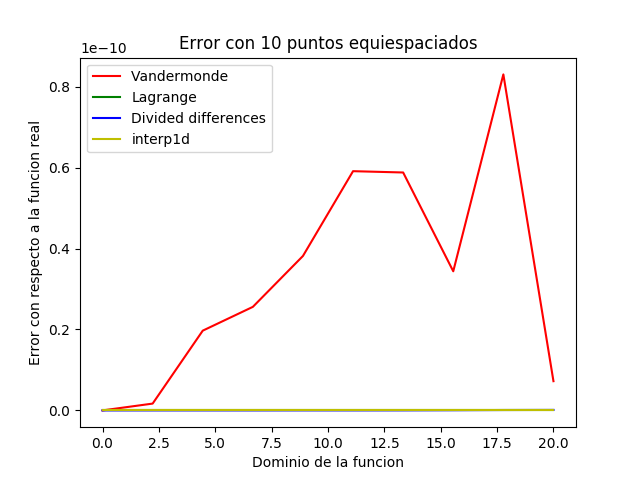
\includegraphics[scale=1.0]{Figure_1.png}

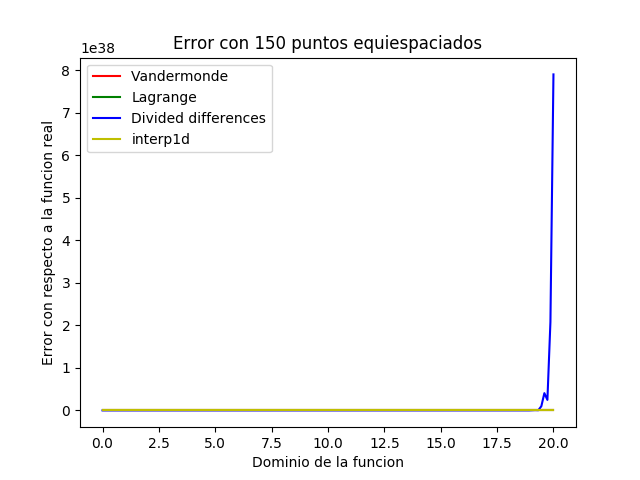
\includegraphics[scale=1.0]{Figure_2.png}

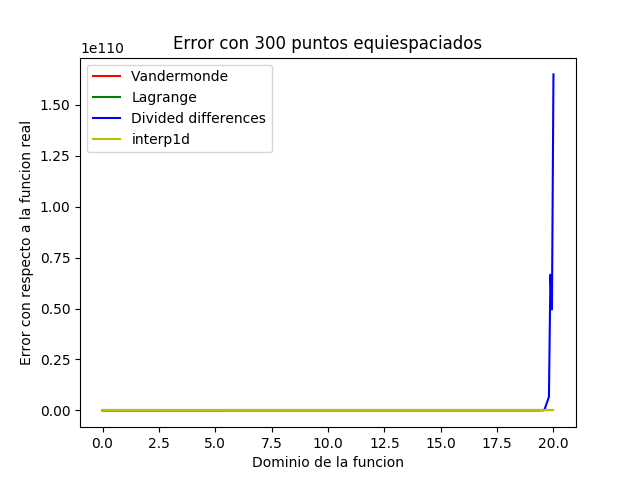
\includegraphics[scale=1.0]{Figure_3.png}

    \item Puntos de \textit{Chevishev}.
    
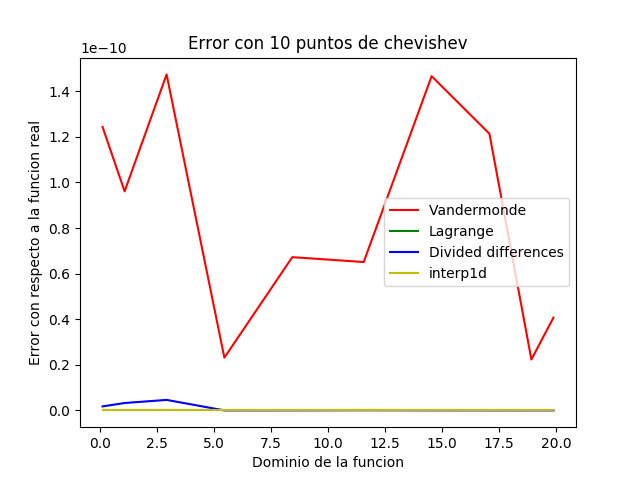
\includegraphics[scale=1.0]{Figure_4.png}

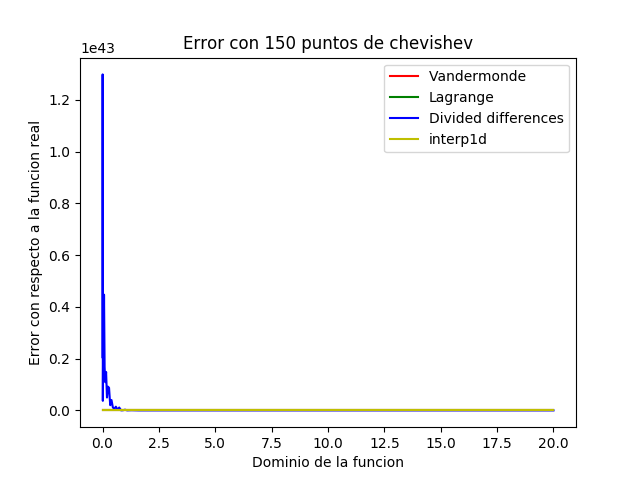
\includegraphics[scale=1.0]{Figure_5.png}

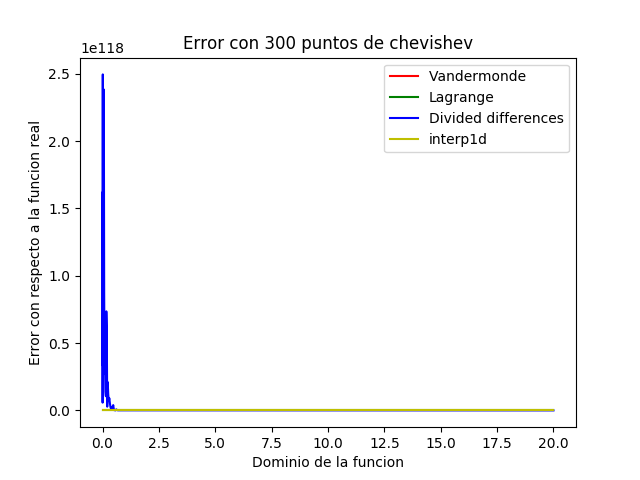
\includegraphics[scale=1.0]{Figure_6.png}
\end{enumerate}

No se que concluir de esto.

En base a los gráficos, mientras mayor sea la cantidad de puntos, mayor es el error resultante entre la función interpolada y la función real.

La diferencia entre usar puntos equiespaciados y \textit{Chevyshev}, en base a estos gráficos, solo mueve el error de un limite del dominio al otro.

Quiero rescatar que, en base a un análisis un poco mas exhaustivo a cada función, tanto \textit{interp1d} como \textit{Lagrange} tienen un error de 0 con respecto a la función real. Esto probablemente se deba a que se están evaluando los mismos puntos con los que se interpolo. Esto es esperado en el caso de \textit{Lagrange} debido a su naturaleza.

\end{document}
